% ........................................................................... %

Timed protocols can be used to model the external behaviors of web services interfaces by capturing the messages choreographies as well as the timing constraints that are put on them. We focus now on the analysis of timed protocols given the following two dimensions: compatibility and replaceability. To do that, we introduce for each type a set of analysis flexible classes. By flexible, we mean that those classes cater for more than ``black or white'' compatibility or replaceability cases like it has been traditionally done for hardware and software components. For example one may look for compatibility or replaceability only for a limited subset of a provider or requester protocol specification.\\

This chapter is structured as follows. We first present compatibility then replaceability analysis before turning our attention to a set of timed protocol operators that can be combined to characterize those classes. The approach that is presented here extends the one from \cite{FTBB} with timing constraints being added to the business protocol model.

% ........................................................................... %

\section{Classes of protocol-based analysis}

% ........................................................................... %

We start this chapter by presenting compatibility then replaceability analysis.

% ........................................................................... %

\subsection{Protocol-level compatibility}

% ........................................................................... %

Compatibility analysis is concerned with verifying whether two services can interoperate. It is necessary for both static and dynamic binding, and it also aids in managing evolution as it helps verify that a modified client can still interact with a certain service.\\

More precisely, we identified two compatibility classes.
\begin{enumerate}

	\item Partial compatibility between two protocols $\mathcal{P}_1$ and $\mathcal{P}_2$ implies that at least one conversation can be carried out between two services implementing these protocols.

  \item A protocol $\mathcal{P}_1$ is \emph{fully compatible} with $\mathcal{P}_2$ if $\mathcal{P}_2$ can support all message exchanges that $\mathcal{P}_1$ can generate (the inverse is not necessarily true).

\end{enumerate}\

Ideally, if we have developed a service $S$ characterized by protocol $\mathcal{P}$, at binding time we will want to look for services that have a protocol with which $\mathcal{P}$ is fully compatible, so that every message exchange that our service can generate is understood by our partner.\\

\begin{figure}[thbp]
    \centering
    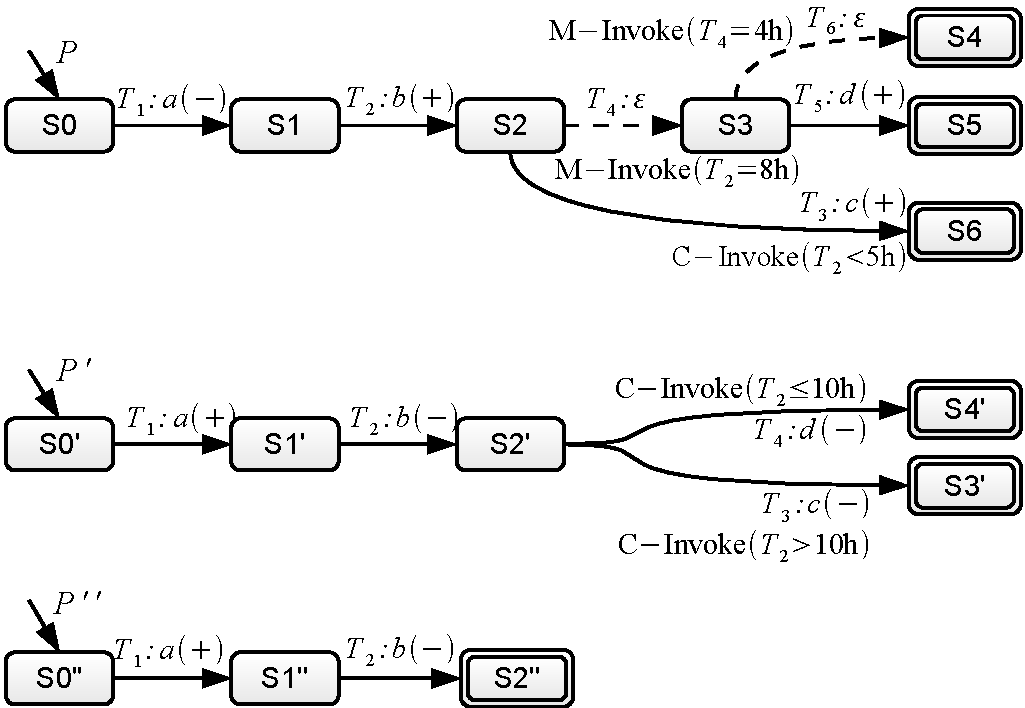
\includegraphics[width=\textwidth]{content/protocol-analysis/analysis}
    \caption{Three protocols for illustrating protocol analysis.}
    \label{fig:analysis}
\end{figure}

We illustrate compatibility analysis with respect to timing constraints and its challenges on the examples below.
Let us consider the protocols $\mathcal{P}$ and $\mathcal{P'}$ depicted on Figure~\ref{fig:analysis}. Without the time constraints, we can observe that $\mathcal{P}$ is fully compatible with $\mathcal{P'}$: $a \cdot b \cdot c$ and
$a \cdot b \cdot d$ are valid interaction traces of the untimed versions of $\mathcal{P}$ and $\mathcal{P'}$. However, due to the \CInvoke constraints specified on transition $T_3$ of each protocol, $\mathcal{P}$ and $\mathcal{P'}$ cannot interact correctly. Indeed, $\mathcal{P}$ supports timed conversations of the form $(a(-), 0) \cdot (b(+), t) \cdot (c(+), t')$ (with $t' < t + 5$), while $\mathcal{P'}$ supports timed conversations of the form $(a(+), 0) \cdot (b(-), t) \cdot (c(-), t')$ (with $t' > t + 10$). Hence, these two protocols cannot interact correctly since $\mathcal{P'}$ will always send a message $c$ later than $\mathcal{P}$ allows it to be received. Therefore, two protocols must agree on the ordering of the exchanged messages as well as on the time constraints to be compatible.\\

Let us now consider the protocols $\mathcal{P}$ and $\mathcal{P''}$ on Figure~\ref{fig:analysis}. When interacting according to the timed interaction trace $(a, 0) \cdot (b, t)$, $\mathcal{P}$ moves to a non-final state $s_2$ while $\mathcal{P''}$ moves to a final state  $s_2''$, ending the conversation from its side. However, due the presence of the implicit transitions $T_4$ and $T_5$, $\mathcal{P}$ is able to terminate correctly its execution by moving automatically to the final state $s_4$: it waits at state $s_2$ for $8$ hours, then moves to $s_3$ where it waits for $4$ hours before finally moving to $s_4$ which is a final state. Therefore, $\mathcal{P}$ and $\mathcal{P''}$ can interact correctly following the interaction trace $(a, 0) \cdot (b, t)$.\\

The last example shows that the implicit transitions have an impact on the identification of the final states, naturally impacting the compatibility analysis. We consider again $\mathcal{P}$ and $\mathcal{P'}$ from Figure~\ref{fig:analysis}.
After exchanging the messages $a$ and $b$, the two protocols move to the states $s_2$ and $s_2'$ respectively. If we consider the explicit operations that are available from these two states, $s_2'$ provides an operation $d(-)$ while $s_2$ does not enable any invocation of a $d$ message receiving operation. As a consequence, focusing the compatibility checking only on these two states is not enough. Indeed, the presence of the implicit transition $T_4$ in $\mathcal{P}$ moves automatically a service conversation to the state $s_3$ after $8$ hours from when $d$ can be received. Hence, $\mathcal{P}$ and $\mathcal{P'}$ can interact correctly by following timed interactions traces of the form $(a, 0) \cdot (b, t) \cdot (c, t')$, with $t + 8 < t' \leq t + 10$ (i.e., if the message $d$ is sent between $8$ and $10$ hours after the message $b$).

% ........................................................................... %

\subsection{Protocol-level replaceability}

% ........................................................................... %

Replaceability analysis identifies whether a service can acts as a substitute of another one, either in general or when interacting with certain requesters. Such an analysis involves finding the set of conversations that both services can support even if they are not equivalent. This is useful, for example, to determine whether a new version of a service (protocol) can support the same conversations as the previous one or whether a newly defined service can support the conversations that a given standard specification mandates.\\

As in the case of compatibility, we identified several replaceability classes.
\begin{enumerate}

	\item \emph{Protocol equivalence} occurs when two protocols support exactly the same conversations.
	
	\item \emph{Protocol subsumption} occurs when a protocol supports at least all of the conversations of another one.
	
	\item \emph{Protocol replaceability w.r.t. a client protocol} occurs when a protocol $\mathcal{P}_1$ can replace a protocol $\mathcal{P}_2$ when interacting with a client protocol $\mathcal{P}_c$ if every valid conversation between $\mathcal{P}_2$ and $\mathcal{P}_c$ is also a valid conversation between $\mathcal{P}_1$ and $\mathcal{P}_c$. This latter definition is helpful in managing evolution, as when we update our service we may want to check that it can still communicate with the same clients it was interacting before.
	
	\item \emph{Protocol replaceability w.r.t. an interaction role} is similar to the previous one. It occurs when a protocol $\mathcal{P}_1$ can replace a protocol $\mathcal{P}_2$ if $\mathcal{P}_1$ behaves like $\mathcal{P}_2$ when $\mathcal{P}_2$ behaves as an interaction role $\mathcal{P}_r$.

\end{enumerate}

For all of the above classes, we can distinguish between full and partial replaceability. Full replaceability is as defined above. Partial replaceability is when there is replaceability but only for some conversations. As an example, we have a partial replaceability with respect to a client protocol when a protocol $\mathcal{P}_1$ can replace another protocol $\mathcal{P}_2$ in at least one conversation that can occur with $\mathcal{P}_c$.\\

To illustrate replaceability, let us consider a protocol $\mathcal{P}_1$ obtained from the protocol $\mathcal{P''}$ on Figure~\ref{fig:analysis} by reversing the polarities of the messages. Such a protocol can be replaced by $\mathcal{P}$ on Figure~\ref{fig:analysis}. Indeed, the only timed conversation supported by  $\mathcal{P}_1$ are of the form $(a(-), 0) \cdot (b(-), t)$ (with $t > 0$) and such  conversations are also supported by  $\mathcal{P}$. The opposite is however not true because for example $\mathcal{P}$ may support some conversations that contain the messages $c$ or $d$, while $\mathcal{P}_1$ does not. Interestingly, we can observe that $\mathcal{P}_1$  can replace $\mathcal{P}$ when interacting with $\mathcal{P''}$: the only timed conversations of $\mathcal{P}$ that are understood by $\mathcal{P''}$ are of the form $(a(-), 0) \cdot (b(-), t)$ (with $t > 0$) and which are also supported by $\mathcal{P}_1$.\\

The next section presents a set of timed protocol operators that can be used to completely characterize the above compatibility and replaceabilty classes.

% ........................................................................... %

\section{Protocol operators}

% ........................................................................... %

We split the set of protocol operators in two categories: \emph{manipulation} and \emph{comparison} operators. The former category allows to compute protocols capturing properties regarding a pair of protocols, for example to compute a protocol that captures all of the common timed conversations of two protocols. The later category allows to compare two protocols for subsumption ($\sqsubseteq$) and equivalence ($\equiv$). We informally describe the protocol manipulation operators below, while their formal semantics are presented in Table~\ref{tab:operators}.

\begin{definition}[Timed protocol operators]
~
\begin{description}

  \item[Parallel composition] ($\compop$) takes two input timed protocols and returns a \emph{timed interaction protocol} that captures the possible interactions between them. A timed interaction protocol has simply no messages polarities. More precisely, the resulting timed interaction protocol describes the set of timed interaction traces of the input protocols.

  \item[Projection] is used to project the polarity of one protocol on the parallel composition of two protocols, and is denoted as $\projop{\mathcal{P}_1}{\mathcal{P}_2}{\mathcal{P}_1}$.

  \item[Intersection] ($\intersop$) takes two input timed protocols and returns one timed protocol that captures the timed conversations that they have in common.

  \item[Difference] ($\diffop$) takes two input timed protocols and returns one that captures the timed conversations that are supported by the first input protocol but not by the second one.
  
  \item[Subsumption] ($\sqsubseteq$) tests whether one protocol supports all of the timed conversations of another protocol (i.e., $\mathcal{P} \sqsubseteq \mathcal{P'}$ if and only if $Tr(\mathcal{P}) \subseteq Tr(\mathcal{P'})$).
  
  \item[Equivalence] ($\equiv$) checks whether two timed protocols support exactly the same set of timed conversations (i.e., $\mathcal{P} \equiv \mathcal{P'}$ if and only if $Tr(\mathcal{P}) = Tr(\mathcal{P'})$. 

\end{description}
\end{definition}

\begin{table}[thbp]
{\footnotesize
\begin{center}
\begin{tabular}{|p{2.5cm}|p{1.2cm}|p{8.3cm}|}
%
\hline
%
\textbf{Operator name} & \textbf{Symbol} &  \textbf{Semantics}\\ \hline
%
Compatible Composition & $\compop$  & $\mathcal{P} = \mathcal{P}_1 \compop \mathcal{P}_2$ is a protocol $\mathcal{P}$ such that
$T \in Tr(\mathcal{P})$ iff  $T$  is an interaction trace of  $\mathcal{P}_1$ and $\mathcal{P}_2$ \\ \hline
%
Intersection  & $\intersop$ & $\mathcal{P} = \mathcal{P}_1 \intersop \mathcal{P}_2$ is a protocol $\mathcal{P}$ such that
$Tr(\mathcal{P}) =  Tr(\mathcal{P}_1) \cap Tr(\mathcal{P}_2)$ \\ \hline
 %
Difference  & $\diffop$ & $\mathcal{P} = \mathcal{P}_1 \diffop \mathcal{P}_2$ is a protocol $\mathcal{P}$ that satisfies the following condition:
$Tr(\mathcal{P}) = Tr(\mathcal{P}_1) \setminus Tr(\mathcal{P}_2) $  \\ \hline
 %
 Projection & $\projop{}{}{}$ &  Let $\mathcal{P} = \mathcal{P}_1 \compop \mathcal{P}_2$. $\projop{\mathcal{P}_1}{\mathcal{P}_2}{\mathcal{P}_i}$, with $i \in \{1, 2\}$,
is the protocol  obtained from $\mathcal{P}_1 \compop \mathcal{P}_2$
by defining  the polarity function of the messages as follows: $Polarity(\projop{\mathcal{P}_1}{\mathcal{P}_2}{\mathcal{P}_i}, m) = Polarity(\mathcal{P}_i, m), \forall m \in \mathtt{M}$ \\ \hline
 %
\end{tabular}
\caption{Protocol manipulation operators semantics.}
\label{tab:operators}
\end{center}
}
\end{table}

\begin{figure}[thbp]
    \centering
    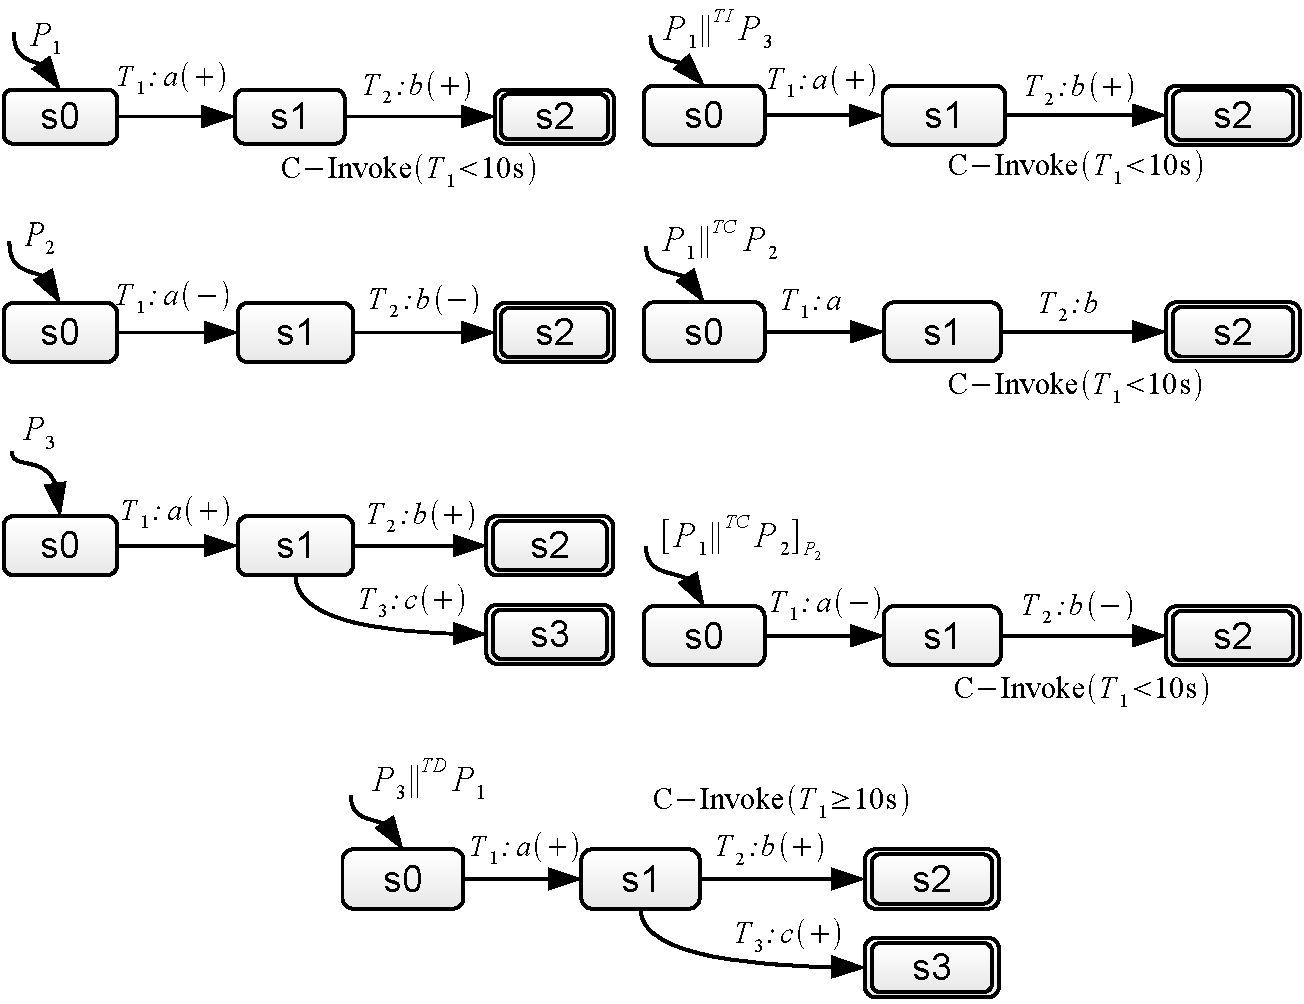
\includegraphics[width=\textwidth]{content/protocol-analysis/operators}
    \caption{Three timed protocols $\mathcal{P}_1, \mathcal{P}_2$ and $\mathcal{P}_3$ and some resulting protocols when using protocol manipulation operators.}
    \label{fig:operators}
\end{figure}

To illustrate these operators, Figure~\ref{fig:operators} shows three simple timed protocols $\mathcal{P}_1$, $\mathcal{P}_2$ and $\mathcal{P}_3$ as well as some results when applying operators on them.
For example, the protocol $\mathcal{P}_1 \intersop \mathcal{P}_3$ captures the timed conversations that are commonly supported by both $\mathcal{P}_1$ and $\mathcal{P}_3$: $\mathcal{P}_1$ does not support receiving a message $c$, hence it does not appear in $\mathcal{P}_1 \intersop \mathcal{P}_3$. Similarly $\mathcal{P}_1$ can only receive a $b$ message within the 10 seconds that follow the reception of a $a$ message. Another example is the protocol $\mathcal{P}_3 \diffop \mathcal{P}_1$ that captures all of the conversations that $\mathcal{P}_3$ supports but that $\mathcal{P}_1$ doesn't support. This is why the \CInvoke constraint of $T_2$ in $\mathcal{P}_3 \diffop \mathcal{P}_1$ is the negation of the one of $T_2$ in $\mathcal{P}_1$ as $\mathcal{P}_3$ does not carry a \CInvoke constraint on its transition $T_2$. Similarly, $\mathcal{P}_3$ supports receiving $c$ messages while $\mathcal{P}_1$ does not. Finally, the protocol $\mathcal{P}_3$ on Figure~\ref{fig:operators} subsumes the protocol $\mathcal{P}_1$.

% ........................................................................... %

\section{Characterizing the compatibility and replaceability classes}

% ........................................................................... %

Based on the operators introduced above, the following lemma gives the necessary and sufficient conditions to identify the compatibility level between two timed protocols.

\begin{lemma}
Let $\mathcal{P}_1$ and $\mathcal{P}_2$ be two timed business protocols.
\begin{enumerate}

    \item $\mathcal{P}_1$ and $\mathcal{P}_2$ are \emph{partially compatible} iff $\mathcal{P}_1 \compop \mathcal{P}_2$ is not an empty protocol (i.e., $Tr(\mathcal{P}_1 \compop \mathcal{P}_2) \neq \emptyset)$).

    \item $\mathcal{P}_1$ and $\mathcal{P}_2$ are \emph{fully compatible} iff $\projop{\mathcal{P}_1}{\mathcal{P}_2}{\mathcal{P}_1} \equiv \mathcal{P}_1$.

\end{enumerate}
\end{lemma}

Indeed, if a timed interaction protocol resulting from a compatible composition of two input protocols is not empty, it means that there is at least one timed interaction trace between the input protocols, and hence these protocols are compatible. Otherwise, the input protocols are not compatible. Regarding the second item of the lemma, the projection $\projop{\mathcal{P}_1}{\mathcal{P}_2}{\mathcal{P}_1}$ describes all the timed conversations of $\mathcal{P}_1$ that are also understood by $\mathcal{P}_2$. As a consequence, if such a set of conversations contains all the ones of $\mathcal{P}_1$, it implies that $\mathcal{P}_1$ is fully compatible with $\mathcal{P}_2$. Otherwise, $\mathcal{P}_1$ is not fully compatible with $\mathcal{P}_2$ since there is at least one timed conversation of $\mathcal{P}_1$ which cannot be understood by $\mathcal{P}_2$.\\

The following lemma characterizes the replaceability levels of two given protocols using the operators introduced in the previous section.

\begin{lemma}
Let $\mathcal{P}_1$, $\mathcal{P}_2$, $\mathcal{P}_C$ and $\mathcal{P}_R$ be three timed business protocols.
\begin{enumerate}

    \item $\mathcal{P}_1$ can \emph{replace} $\mathcal{P}_2$ iff $\mathcal{P}_2 \sqsubseteq \mathcal{P}_1$.

    \item $\mathcal{P}_1$ and $\mathcal{P}_2$ are \emph{equivalent} w.r.t. replaceability iff $\mathcal{P}_1 \equiv \mathcal{P}_2$.

    \item $\mathcal{P}_1$ can replace $\mathcal{P}_2$ w.r.t. a \emph{client protocol} $\mathcal{P}_C$ iff $\projop{\mathcal{P}_C}{\mathcal{P}_2}{\mathcal{P}_2} \sqsubseteq \mathcal{P}_1$ (or equivalently iff
$\mathcal{P}_C \compop (\mathcal{P}_2 \diffop \mathcal{P}_1)$ is an empty protocol).

    \item $\mathcal{P}_1$ can replace $\mathcal{P}_2$ w.r.t. a \emph{role} $\mathcal{P}_R$ iff $(\mathcal{P}_R \intersop \mathcal{P}_2) \sqsubseteq \mathcal{P}_1$.

\end{enumerate}
\end{lemma}

The characterization of the subsumption and equivalence w.r.t. replaceability is immediate. Regarding the third class of replaceability, the lemma defines that if all of the timed conversations of a protocol $\mathcal{P}_1$ that are also understood by a protocol $\mathcal{P}_C$ (given by the projection of $\mathcal{P}_1$ on compatible composition of $\mathcal{P}_1$ and $\mathcal{P}_C$) are compliant with a protocol $\mathcal{P}_2$, then $\mathcal{P}_2$ can replace $\mathcal{P}_1$ when interacting with $\mathcal{P}_C$. Finally, the last item of the lemma defines that if the common timed conversations of $\mathcal{P}_2$ and $\mathcal{P}_R$ (given by the intersection of $\mathcal{P}_2$ and $\mathcal{P}_R$) are compliant with $\mathcal{P}_1$ then $\mathcal{P}_1$ can replace $\mathcal{P}_2$ when  $\mathcal{P}_2$ behave as $\mathcal{P}_R$.\\

\begin{table}[tbhp]
  \footnotesize
  \begin{center}
  \begin{tabular}{|p{0.46\textwidth}|p{0.46\textwidth}|}
    
    \hline
    
    \textbf{Class} & \textbf{Characterization}
    \\ \hline
    
    Partial compatibility of $\mathcal{P}_1$ and $\mathcal{P}_2$ &
    $\mathcal{P}_1 \compop \mathcal{P}_2$ is not \emph{empty}
    \\ \hline
    
    Full compatibility of $\mathcal{P}_1$ and $\mathcal{P}_2$ &
    $\projop{\mathcal{P}_1}{\mathcal{P}_2}{\mathcal{P}_1} \equiv \mathcal{P}_1$
    \\ \hline
    
    Replaceability of $\mathcal{P}_1$ by $\mathcal{P}_2$ &
    $\mathcal{P}_2 \sqsubseteq \mathcal{P}_1$
    \\ \hline
    
    Equivalence of $\mathcal{P}_1$ and $\mathcal{P}_2$ w.r.t. replaceability &
    $\mathcal{P}_1 \equiv \mathcal{P}_2$
    \\ \hline
    
    Replaceability of $\mathcal{P}_2$ by $\mathcal{P}_1$ w.r.t. a client protocol $\mathcal{P}_C$ &
    $\projop{\mathcal{P}_C}{\mathcal{P}_2}{\mathcal{P}_2} \sqsubseteq \mathcal{P}_1$ or equivalently
    $\mathcal{P}_C \compop (\mathcal{P}_2 \diffop \mathcal{P}_1)$ is \emph{empty}
    \\ \hline
    
    Replaceability of $\mathcal{P}_2$ by $\mathcal{P}_1$ w.r.t. a role $\mathcal{P}_R$ &
    $(\mathcal{P}_R \intersop \mathcal{P}_2) \sqsubseteq \mathcal{P}_1$
    \\ \hline
    
  \end{tabular}
  \end{center}
  \caption{Characterization of the compatibility and replaceability classes.}
  \label{tab:classes-characterization}
\end{table}

We have summarized the operators-based characterization of the compatibility and replaceability classes in Table~\ref{tab:classes-characterization}.\\

\begin{figure}[tbhp]
    \centering
    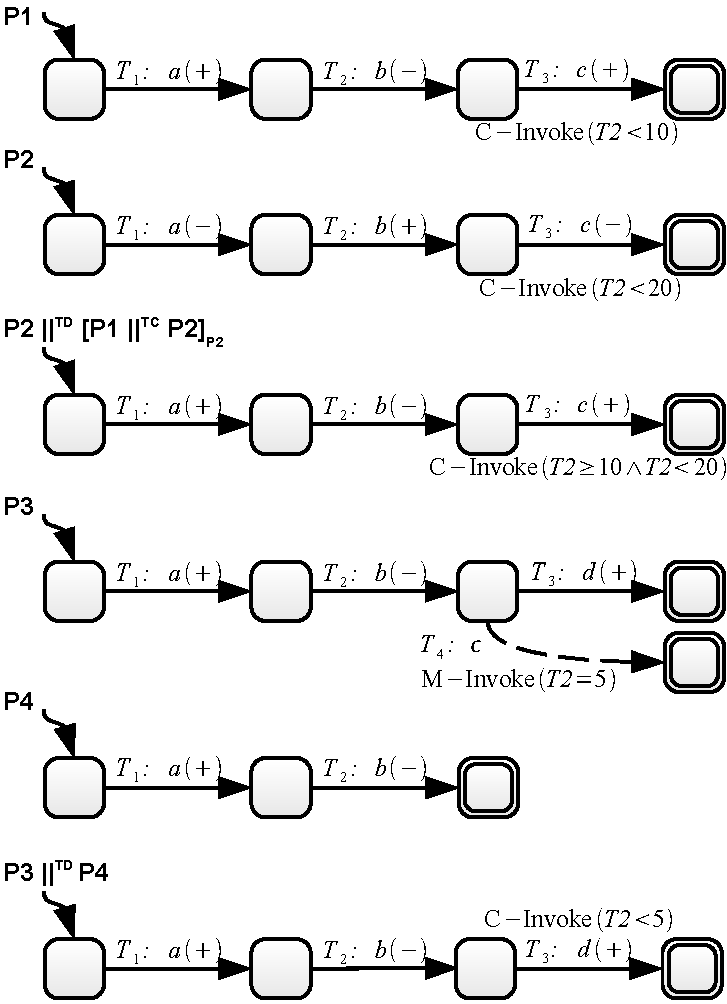
\includegraphics[width=0.8\textwidth]{content/protocol-analysis/compat-and-diff}
    \caption{Compatibility and replaceability analysis.}
    \label{fig:compat-and-diff}
\end{figure}

We give examples of operators-based compatibility and replaceability analysis on Figure~\ref{fig:compat-and-diff}. $\mathcal{P}_1$ and $\mathcal{P}_2$ are only partially compatible, as
$$ \projop{\mathcal{P}_1}{\mathcal{P}_2}{\mathcal{P}_2} \not\equiv \mathcal{P}_2 $$
By using the difference operator to compute $\mathcal{P}_2 \diffop \projop{\mathcal{P}_1}{\mathcal{P}_2}{\mathcal{P}_2}$, we get the set of conversations that are supported by $\mathcal{P}_2$ but not by $\mathcal{P}_1$ which yield to a partial compatibility ($\mathcal{P}_1$ does not support receiving a $c$ message after 10 units of time). $\mathcal{P}_4$ can be replaced by $\mathcal{P}_3$ as it supports all of the conversations that $\mathcal{P}_4$ supports: $\mathcal{P}_3 \sqsubseteq \mathcal{P}_4$. The converse is however not true as illustrated by $\mathcal{P}_3 \diffop \mathcal{P}_4$: $\mathcal{P}_3$ cannot handle $d$ messages.

% ........................................................................... %

\section{Discussion}

% ........................................................................... %

We briefly review the related work and discuss the limitations regarding the message-level matching that is performed in our approach.

% ........................................................................... %

\subsection{Related work}

% ........................................................................... %

\subsubsection{Verification techniques}

% ........................................................................... %

Many works in various fields have applied verification techniques such as checking for liveness, the absence of deadlocks or the conformance against specifications.
%
A substantial amount of work has been done in the field of workflow systems \cite{aalst98application,DMMZ06,BWJ02}.
In the case of web services, timed automata have been used in \cite{KazhamiakinPP06,DCPVC06}. In  \cite{berardi03finite} the introduced WSTL model had been designed with timing constraints as ``first-class citizen''. The analysis techniques presented in this paper did not leverage the timing constraints though, and while this had been mentioned as future work, it hasn't yet been done.\\

BPEL-based web services interactions have been analyzed in \cite{FBS04} by the mean of guarded automata with unbounded message queues where the automata synchronizablility problem is studied in synchronous and asynchronous communications.
Formal verification of service compositions is the target of several works: \cite{RouachedPG06,Bultan03,GLTXH07,FUMK03}.
The same types of verifications can be performed on protocol timed automata using TCTL, an extension of temporal logics for timed automata, and a model checker such as UPPAAL \cite{UPPAAL}.

% ........................................................................... %

\subsubsection{Compatibility and replaceability}

% ........................................................................... %

Software components have some fundamental similarities with web services: they promote good practices such as loose coupling and reuse. Also, they can be remotely accessed over a network. Similar approaches for protocols compatibility and replace-ability exist in the area of component-based systems \cite{Yellin97,CCLF+06}.\\

The importance of being able to check for services compatibility or replace-ability has lead to several research works \cite{MPC-TES01,FUMK-OE05,DBACTH05}. Surprisingly, these approaches do not cater for timing constraints.\\

They also perform ``black or white'' analysis. By contrast, our approach is able to provide a more fine-grained type of analysis by identifying the ``partial cases'' like the partial compatibility or the replace-ability with respect to a client protocol. We believe that this flexibility will significantly prove to be useful in practice, as full compatibility or replace-ability of business protocols can hardly be reached on the Internet which is an open service deployment environment.\\

The notion of process inheritance has been studied in the domain of workflows \cite{aalst03inheritance,Bussler02}. It is similar to protocols replaceability. Different types of inheritance relations are proposed in \cite{aalst03inheritance}. They provide some flexibility much like we did with the different classes of protocol replaceability. However, these approaches do not consider temporal abstractions.

% ........................................................................... %

\subsubsection{Model management}

% ........................................................................... %

The work that has been done in the model management area focuses on manipulating models (e.g., database schemas, XML schemas) and matches between them (e.g., equivalence between 2 database schema) on an equal foot \cite{BMPQ-SGR04}. The matches relationships between 2 models can be used for matching, merging or composition purposes. The models can also be manipulated through various operators like the intersection, the union or the difference.\\

A set of combined static and behavioral matching and merging techniques for statecharts-based specifications have been proposed in \cite{NSEZ-ICSE07}. This work has been done in a similar fashion as the approaches for schema matching (including databases and XML) mentioned in \cite{ERPB-VLDBJ01,BMPQ-SGR04}.\\

The work presented in this thesis shares some analogies with what has been done in this research field. Indeed, timed protocol is a model for which there exist protocol manipulation operators (composition, difference and intersection) as well as comparison operators (subsumption and equivalence).

% ........................................................................... %

\subsection{Message matching}

Our approach is mainly ``syntactic'' in the sense that when considering two messages named $\mathtt{login}$, we assume that both their schema and semantics are identical. This is of course not always the case in reality. As far as the schema is concerned, a better way for comparing two messages in the protocol operators would be to also look at their definitions (e.g., in XML Schema, grabbed from the services WSDL specifications). To do that, we could reuse schema matching algorithms as studied in \cite{ERPB-VLDBJ01,BMPQ-SGR04} or the approach presented in \cite{DongHMNZ04} which is more specific to web services interfaces. In some cases an adapter could be generated at the static interface level (messages schema and operations). \\

Another limit of the way that the messages matching is performed is that 2 messages $\mathtt{login}$ and $\mathtt{logUserIn}$ are considered to be different, although they could have exactly the same schema and/or semantics (or both could be ``close'' enough for easy adaptation). A potential solution would be to integrate the \emph{match} operator presented in \cite{NSEZ-ICSE07} with our compatibility and replaceability analysis techniques as it addresses such type of issues. The operator uses a heuristic that requires human intervention for identifying missing and invalid matches. If such an approach turned out to be useful, the identified message matches and mismatches could then be exploited to generate protocol adapters \cite{BenatallahCGNT05,MBMCC-WWW07}.

% ........................................................................... %